\documentclass[../book.tex]{subfiles}
\graphicspath{{\subfix{../images/}}}

\begin{document}
\chapter{Trigonometry}
\begin{introduction}[Contents]
\item The Trigonometric Functions
\item The Unit Circle
\item Solving Trigonometric Equations
\item Graphing Trigonometric Functions
\item Author's Note on Sinusoidal Curves
\end{introduction}
\noindent Well, here we are, trigonometry $-$ what for many Americans is the summit of their mathematical adventure. To keep things relatively simple, we will only be providing an introduction into the field, as the full extent of it will be covered later on during your time in Pre-calculus. Technically, trigonometry is the study of triangles, coming from the roots "tri" for $3$ (sides/angles) and “metry” meaning to measure. In practice, however, trigonometry more often involves the study of certain \textit{trigonometric functions} which enable greater understanding of both triangles and a wide variety of other applications. As you will soon find out, to understand and intuit in place of memorize, trigonometry will often require of you a certain flexibility $-$ to be able to quickly switch between algebraic and geometric perspectives.  
\section{The Trigonometric Functions}
\noindent We'll start with the very basics. First, since this chapter is about trigonometry, let's look at some simple cases of triangles. Let's say we have a right triangle and we know one of the (non-right) angles. For the sake of simplicity, let's also assume we know the hypotenuse has a length of one. Below are some cases of the above situation:
\begin{figure}[!ht]
    \centering
    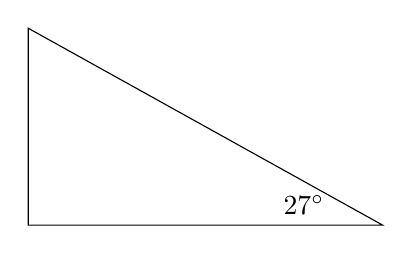
\begin{tikzpicture}[xscale=0.5,yscale=0.5]
        \draw (0,0) -- (9,0) -- (0,5) -- cycle;
        \draw (7,0.5) node {$27^{\circ}$};
    \end{tikzpicture}
    \hspace{0.5cm}
    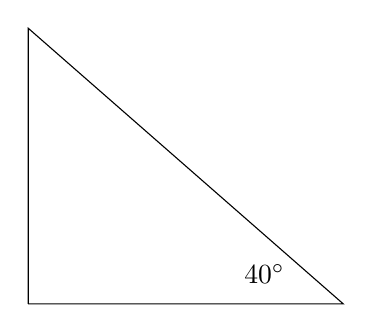
\begin{tikzpicture}[xscale=0.5,yscale=0.5]
        \draw (0,0) -- (0,7) -- (8,0) -- (0,0);
        \draw (6,0.75) node {$40^{\circ}$};
    \end{tikzpicture}
    \hspace{0.5cm}
    \begin{tikzpicture}[xscale=0.5,yscale=0.5]
        \draw (0,0) -- (90:7cm) -- (0:7cm) -- (0,0);
        \draw (5,0.6) node {$45^{\circ}$};
    \end{tikzpicture}
\end{figure}
In these examples, it would be incredibly difficult (if not near impossible) to calculate the length of the other two sides of the triangle. So, in an attempt to make some progress, let's create some functions $f(\theta)$ and $g(\theta)$ to help us with these cases. $f(\theta)$ will take the known angle $\theta$ as an input to the function and output the length of the side of the triangle \textit{opposite} the angle $\theta$; likewise, $g(\theta)$ will take the known angle $\theta$ as an input and output the length of the side of the triangle \textit{adjacent} the angle $\theta$.

We can observe the general case for this situation below with the known angle $\theta$ and lengths $1$, $f(\theta)$,and $g(\theta)$: \newpage
\begin{figure}
    \centering
    \hspace{\stretch{1}}
    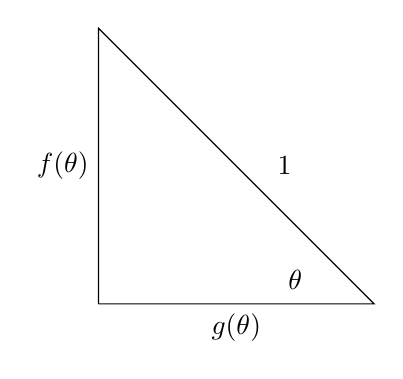
\begin{tikzpicture}[xscale=0.5,yscale=0.5]
        \draw (0,0) -- (90:7cm) node[midway,left] {$f(\theta)$} -- (0:7cm) node[midway,right=0.4cm] {$1$} -- (0,0) node[midway,below] {$g(\theta)$};
        \draw (5,0.6) node {$\theta$};
    \end{tikzpicture}
    \hspace{\stretch{1}}
    \begin{tikzpicture}[xscale=0.5,yscale=0.5]
        \draw (0,0) -- (90:7cm) node[midway,left] {$g(\theta)$} -- (0:7cm) node[midway,right=0.4cm] {$1$} -- (0,0) node[midway,below] {$f(\theta)$};
        \draw (0.65,5.2) node {$\theta$};
    \end{tikzpicture}
    \hspace{\stretch{1}}
\end{figure}
Now it just so happens that these functions are useful enough to where mathematicians have given these two functions special names. $f(\theta)$, the length of the side opposite the angle, is denoted by $\sin(\theta)$; $g(\theta)$, the length of the side adjacent the angle, is denoted by $\cos(\theta)$.
\begin{note}
From here on, $\sin(\theta)$ and $\cos(\theta)$ will be used in place of $f(\theta)$ and $g(\theta)$.  All trigonometric functions will take $\theta$ to be in \textit{radians} instead of \textit{degrees}.
\end{note}
Now that we have all the setup in place, let's try and calculate some simple cases of $\sin(\theta)$ and $\cos(\theta)$. While you may not be expected to derive some of these without having seen the proof beforehand, it is recommended that you understand them regardless.
\begin{example}
Using principles of geometry, calculate $\sin(0)$ and $\cos(0)$.
\end{example}
\begin{solution}
Consider the left triangle above.  As $\theta$ approaches $0$, we see that $f(0)=\sin(0)$ approaches $0$. Using the Pythagorean Theorem (or similar logic to $\sin(\theta)$ we see that $g(0)=\cos(0)$ approaches $1$. $\Box$
\end{solution}
Here are the figures for the next two problems.  Due to spacing limitations, we were forced to put them above.
\begin{figure}[!ht]
    \centering
    \hspace{\stretch{1}}
    \begin{tikzpicture}[xscale=0.5,yscale=0.5]
        \draw (0,0) -- (90:7cm) node[midway,left] {$A$} -- (0:7cm) node[midway,right=0.4cm] {$1$} -- (0,0) node[midway,below] {$B$};
        \draw (0.65,5.2) node {$\theta$};
        \draw (5,0.6) node {$\phi$};
    \end{tikzpicture}
    \hspace{\stretch{1}}
    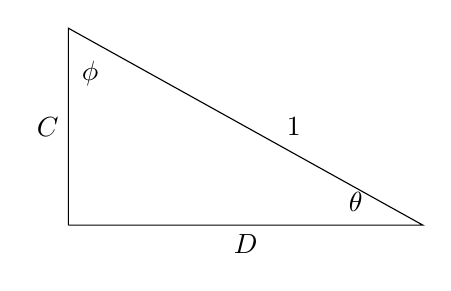
\begin{tikzpicture}[xscale=0.5,yscale=0.5]
        \draw (0,0) -- (90:5cm) node[midway,left] {$C$} -- (0:9cm) node[midway,right=0.4cm] {$1$} -- (0,0) node[midway,below] {$D$};
        \draw (0.55,3.85) node {$\phi$};
        \draw (7.3,0.6) node {$\theta$};
    \end{tikzpicture}
    \hspace{\stretch{1}}
\end{figure}


\begin{example}
Using principles of geometry, calculate $\sin\left(\dfrac{\pi}{4}\right)$ and $\cos\left(\dfrac{\pi}{4}\right)$.
\end{example}
\begin{solution}
Consider the triangle to the right. We know that the sum of the angles in a triangle must add up to $180^{\circ}$ (or $\pi$), so we know that $\theta=\phi=\dfrac{\pi}{4}$.  This also tells us that $A=B$ (from one of those theorems from Geometry $-$ it says that side lengths are proportional to their angle measure).

Using the Pythagorean Theorem, we can say the following: $$A^2+B^2=1 \implies A^2+A^2=1 \implies A^2=\dfrac{1}{2} \implies A=\dfrac{\sqrt{2}}{2}.$$ This means that we can conclude that $$\sin\left(\dfrac{\pi}{4}\right)=\cos\left(\dfrac{\pi}{4}\right)=\dfrac{\sqrt{2}}{2}.$$ $\Box$
\end{solution}
\begin{remark}
Note that in the example above we didn't accept the negative solution for $A$.  We can't have negative lengths.
\end{remark}
\begin{example}
Using principles of geometry, calculate $\sin\left(\dfrac{\pi}{6}\right)$ and $\cos\left(\dfrac{\pi}{6}\right)$.
\end{example}
\begin{solution}
Based on the diagram to the right, let's set $\phi$ to equal $\frac{\pi}{6}$. Then, we know $\sin\left(\dfrac{\pi}{6}\right)=D$ and $\cos\left(\dfrac{\pi}{6}\right)=C$.

Since all angles in the triangle must add to $\pi$, we calculate $\theta$ to be $\theta=\dfrac{\pi}{2}-\dfrac{\pi}{6}=\dfrac{\pi}{3}.$

Here's where the clever trick gets involved, notice how $2\phi=\theta$. This fact allows us to leverage some symmetry. The “trick” for this problem is to add a second triangle to the diagram as shown below.
\begin{figure}[!ht]
    \centering
    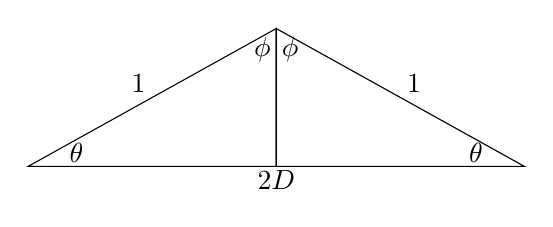
\begin{tikzpicture}[xscale=0.35,yscale=0.35]
        \draw (-9,0) -- (0,0) -- (0,5) -- cycle;
        \draw (0,0) -- (9,0) -- (0,5) -- cycle;
        \draw (-7.25,0.5) node {$\theta$};
        \draw (7.25,0.5) node {$\theta$};
        \draw (-0.5,4.25) node {$\phi$};
        \draw (0.5,4.25) node {$\phi$};
        \draw (0,-0.5) node {$2D$};
        \draw (5,3) node {$1$};
        \draw (-5,3) node {$1$};
    \end{tikzpicture}
    \hspace{\stretch{1}} $\to$ \hspace{\stretch{1}}
    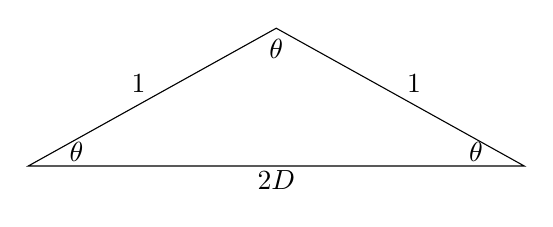
\begin{tikzpicture}[xscale=0.35,yscale=0.35]
        \draw (-9,0) -- (9,0) -- (0,5) -- cycle;
        \draw (0,4.25) node {$\theta$};
        \draw (-7.25,0.5) node {$\theta$};
        \draw (7.25,0.5) node {$\theta$};
        \draw (0,-0.5) node {$2D$};
        \draw (5,3) node {$1$};
        \draw (-5,3) node {$1$};
    \end{tikzpicture}
\end{figure}

By adding on a second triangle we can form one larger triangle with equal angles, an equilateral, and therefore we know all of the side lengths must be equal. This means that $2D=1$, or $D=\dfrac{1}{2}$.

Since we know two out of the three side lengths of the original triangle, we can use the Pythagorean Theorem again. $$C^2+\left(\dfrac{1}{2}\right)^2=1 \implies C^2=\dfrac{3}{4} \implies C=\dfrac{\sqrt{3}}{2}.$$ We can use the definitions for $C$ and $D$ established above to say that $\sin\left(\dfrac{\pi}{6}\right)=\dfrac{1}{2}$ and $\cos\left(\dfrac{\pi}{6}\right)=\dfrac{\sqrt{3}}{2}$. $\Box$
\end{solution}
What if we have a right triangle with a hypotenuse not equal to $1$ and we want to know the lengths of the other sides? Well, we can use a simple property regarding similar triangles.

\begin{figure}
    \centering
    \hspace{\stretch{1}}
    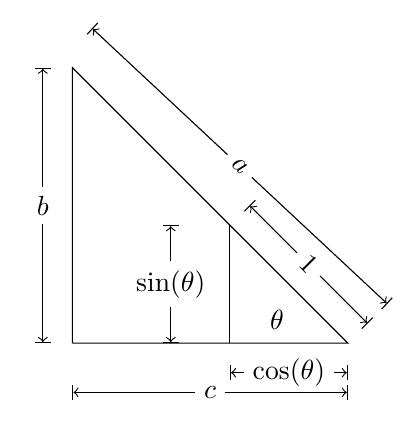
\begin{tikzpicture}[xscale=0.5,yscale=0.5]
        \draw (0,0) -- (90:7cm) -- (0:7cm) -- (0,0);
        \draw (4,0) -- (4,3);
        \draw (5.2,0.6) node {$\theta$};
        \draw[|<->|] (4,-0.75) -- node[fill=white,sloped] {$\cos(\theta)$} (7,-0.75);
        \draw[|<->|] (0,-1.25) -- node[fill=white,sloped] {$c$} (7,-1.25);
        \draw[|<->|] (0.5,8) -- node[fill=white,sloped] {$a$} (8,1);
        \draw[|<->|] (4.5,3.5) -- node[fill=white,sloped] {$1$} (7.5,0.5);
        \draw[|<->|] (-0.75,0) -- node[fill=white] {$b$} (-0.75,7);
        \draw[|<->|] (2.5,0) -- node[fill=white] {$\sin(\theta)$} (2.5,3);
    \end{tikzpicture} \hspace{\stretch{1}} $\to$ \hspace{\stretch{1}}
    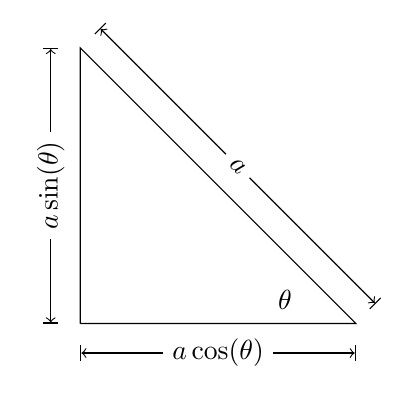
\begin{tikzpicture}[xscale=0.5,yscale=0.5]
        \draw (0,0) -- (90:7cm) -- (0:7cm) -- (0,0);
        \draw (5.2,0.6) node {$\theta$};
        \draw[|<->|] (0,-0.75) -- node[fill=white,sloped] {$a\cos(\theta)$} (7,-0.75);
        \draw[|<->|] (0.5,7.5) -- node[fill=white,sloped] {$a$} (7.5,0.5);
        \draw[|<->|] (-0.75,0) -- node[fill=white,sloped] {$a\sin(\theta)$} (-0.75,7);
    \end{tikzpicture}
    \hspace{\stretch{1}}
\end{figure}



Since these two triangles share all the same angles, we automatically know the triangles are similar to each other.  This is seen in the figure to the left at the top of the next page.  One property of similar triangles is that equivalent sides are proportional: $$\dfrac{a}{1}=\dfrac{b}{\sin(\theta)}=\dfrac{c}{\cos(\theta)}\implies \begin{matrix} b=a\cdot\sin(\theta) \\c=a\cdot\cos(\theta) \end{matrix}.$$ Substituting in these values for the leg side lengths, we see that each leg is scaled by the length of the hypotenuse. This is seen in the figure on the right.  \newpage

We can now create our formal definitions for $\sin(\theta)$ and $\cos(\theta)$ using the substitutions we made.  We see that $$\sin(\theta)=\dfrac{b}{a}=\dfrac{\text{\textit{opposite}}}{\text{\textit{hypotenuse}}} \hspace{15mm} \cos(\theta)=\dfrac{c}{a}=\dfrac{\text{\textit{adjacent}}}{\text{\textit{hypotenuse}}}.$$

We have four more functions you need to know. These, however, are much easier to learn about as they all are simple combinations of the sine and cosine functions.

Let's start with $\tan(\theta)$ (short for "tangent"). By definition, $\tan(\theta)=\dfrac{\sin(\theta)}{\cos(\theta)}$. In addition to this algebraic definition, the tangent function may also be defined geometrically. The tangent of an angle can be found by taking the ratio between the opposite and adjacent legs of the triangle: $\tan(\theta)=\dfrac{\text{\textit{opposite}}}{\text{\textit{adjacent}}}$.

\begin{remark}
the length of the hypotenuse does not matter when calculating the tangent (it does with Sine and Cosine, which will be covered in section 13.2).
\end{remark}

The final three functions are the reciprocals of the first three: cosecant the reciprocal of sine, secant of cosine, and cotangent of tangent. $$\csc(\theta)=\dfrac{1}{\sin(\theta)} \hspace{15mm} \sec(\theta)=\dfrac{1}{\cos(\theta)}\hspace{15mm} \cot(\theta)=\dfrac{1}{\tan(\theta)}.$$

While these three tend to have less applications, they are certainly useful as a shorthand in place of writing out the reciprocals whenever they come up.

\section{The Unit Circle}
\begin{wrapfigure}{r}{4cm}
    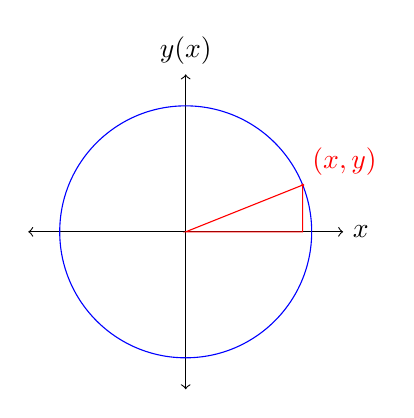
\begin{tikzpicture}[xscale=0.20,yscale=0.20]
      \draw[<->] (-10,0) -- (10,0) node[right] {$x$};
      \draw[<->] (0,-10) -- (0,10) node[above] {$y(x)$};
      \draw[blue] (0,0) circle[radius=8];
      \draw[red] (0,0) -- (7.428,2.971) -- (7.428,0) -- cycle;
      \filldraw[red] (7.428,2.971) circle[radius=1.5pt] node[anchor=south west] {$(x,y)$};
    \end{tikzpicture}
\end{wrapfigure}
\noindent It is often said that when you start out in trigonometry you think it's all about triangles, but in actuality, it's all about circles.

In this section we are going to flesh out a more useful definition to the sine and cosine functions to that of the previous one based on the length of a triangle's side. The first thing we want to improve with our new definition is to be able to \textit{extend the domain} of each function. With the triangle definition we couldn't reasonably define a value to $\sin\left(\dfrac{3\pi}{2}\right)$ or $\cos(10\pi)$, that would imply it is possible to have a right triangle with an angle of $\dfrac{3\pi}{2}$ or $10\pi$ (which is impossible due to the sum to $\pi$ rule). Currently our domain is limited to an angle theta in the interval $\left[0,\dfrac{\pi}{2}\right)$, we want it to range over $\mathbb{R}$.

In the diagram at the beginning of the section, we have a general point $(x,y)$ on a unit circle (circle of radius of one and centered at the origin). We can form a right triangle within this unit circle with the points $(x,y)$, $(0,0)$, and some other point found by dropping a vertical from $(x,y)$ onto the $x$-axis.

Let the angle between the hypotenuse and horizontal leg of the triangle be denoted by $\theta$. Since we know the radius is one, we know the opposite leg (with length $y$) equals $\sin(\theta)$, while the adjacent leg (with length $x$) is equal to $\cos(\theta)$.

This diagram will lead us to our new definitions. Let $\sin(\theta)$ be equal to the $y$-coordinate of the point found by walking theta radians around a unit circle (counterclockwise); $\cos(\theta)$ is the same, but the $x$-coordinate. Negative angles will be computed by performing a clockwise rotation.
\begin{figure}[!ht]
\centering
    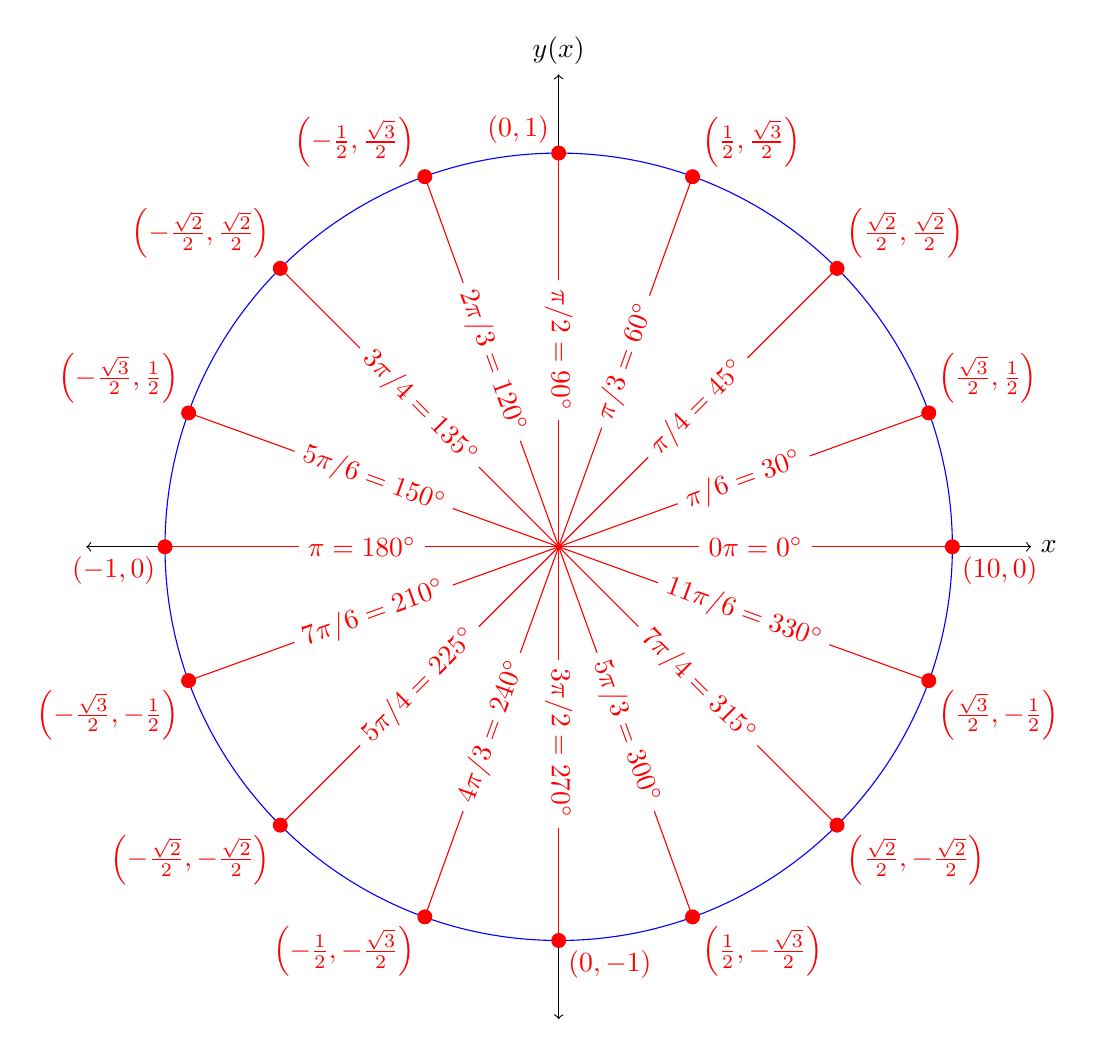
\begin{tikzpicture}[xscale=0.5,yscale=0.5]
      \draw[<->] (-12,0) -- (12,0) node[right] {$x$};
      \draw[<->] (0,-12) -- (0,12) node[above] {$y(x)$};
      \draw[blue] (0,0) circle[radius=10];
      
      \draw[red] (0,0) -- node[fill=white,midway,sloped] {$\pi/6=30^{\circ}$} (9.4,3.4);
      \filldraw[red] (9.4,3.4) circle[radius=5pt] node[anchor=south west] {$\left(\frac{\sqrt{3}}{2},\frac{1}{2}\right)$};
      
      \draw[red] (0,0) -- node[fill=white,midway,sloped] {$\pi/4=45^{\circ}$} (7.071,7.071);
      \filldraw[red] (7.071,7.071) circle[radius=5pt] node[anchor=south west] {$\left(\frac{\sqrt{2}}{2},\frac{\sqrt{2}}{2}\right)$};
      
      \draw[red] (0,0) -- node[fill=white,midway,sloped] {$\pi/3=60^{\circ}$} (3.4,9.4);
      \filldraw[red] (3.4,9.4) circle[radius=5pt] node[anchor=south west] {$\left(\frac{1}{2},\frac{\sqrt{3}}{2}\right)$};
      
      \draw[red] (0,0) -- node[fill=white,midway,sloped] {$0\pi=0^{\circ}$} (10,0);
      \filldraw[red] (10,0) circle[radius=5pt] node[anchor=north west] {$\left(10,0\right)$};
      
      \draw[red] (0,10) -- node[fill=white,midway,sloped] {$\pi/2=90^{\circ}$} (0,0);
      \filldraw[red] (0,10) circle[radius=5pt] node[anchor=south east] {$\left(0,1\right)$};
      
      \draw[red] (-10,0) -- node[fill=white,midway,sloped] {$\pi=180^{\circ}$} (0,0);
      \filldraw[red] (-10,0) circle[radius=5pt] node[anchor=north east] {$\left(-1,0\right)$};
      
      \draw[red] (-9.4,3.4) -- node[fill=white,midway,sloped] {$5\pi/6=150^{\circ}$} (0,0);
      \filldraw[red] (-9.4,3.4) circle[radius=5pt] node[anchor=south east] {$\left(-\frac{\sqrt{3}}{2},\frac{1}{2}\right)$};
      
      \draw[red] (-7.071,7.071) -- node[fill=white,midway,sloped] {$3\pi/4=135^{\circ}$} (0,0);
      \filldraw[red] (-7.071,7.071) circle[radius=5pt] node[anchor=south east] {$\left(-\frac{\sqrt{2}}{2},\frac{\sqrt{2}}{2}\right)$};
      
      \draw[red] (-3.4,9.4) -- node[fill=white,midway,sloped] {$2\pi/3=120^{\circ}$} (0,0);
      \filldraw[red] (-3.4,9.4) circle[radius=5pt] node[anchor=south east] {$\left(-\frac{1}{2},\frac{\sqrt{3}}{2}\right)$};
      
      \draw[red] (-9.4,-3.4) -- node[fill=white,midway,sloped] {$7\pi/6=210^{\circ}$} (0,0);
      \filldraw[red] (-9.4,-3.4) circle[radius=5pt] node[anchor=north east] {$\left(-\frac{\sqrt{3}}{2},-\frac{1}{2}\right)$};
      
      \draw[red] (-7.071,-7.071) -- node[fill=white,midway,sloped] {$5\pi/4=225^{\circ}$} (0,0);
      \filldraw[red] (-7.071,-7.071) circle[radius=5pt] node[anchor=north east] {$\left(-\frac{\sqrt{2}}{2},-\frac{\sqrt{2}}{2}\right)$};
      
      \draw[red] (-3.4,-9.4) -- node[fill=white,midway,sloped] {$4\pi/3=240^{\circ}$} (0,0);
      \filldraw[red] (-3.4,-9.4) circle[radius=5pt] node[anchor=north east] {$\left(-\frac{1}{2},-\frac{\sqrt{3}}{2}\right)$};
      
      \draw[red] (0,0) -- node[fill=white,midway,sloped] {$11\pi/6=330^{\circ}$} (9.4,-3.4);
      \filldraw[red] (9.4,-3.4) circle[radius=5pt] node[anchor=north west] {$\left(\frac{\sqrt{3}}{2},-\frac{1}{2}\right)$};
      
      \draw[red] (0,0) -- node[fill=white,midway,sloped] {$7\pi/4=315^{\circ}$} (7.071,-7.071);
      \filldraw[red] (7.071,-7.071) circle[radius=5pt] node[anchor=north west] {$\left(\frac{\sqrt{2}}{2},-\frac{\sqrt{2}}{2}\right)$};
      
      \draw[red] (0,0) -- node[fill=white,midway,sloped] {$5\pi/3=300^{\circ}$} (3.4,-9.4);
      \filldraw[red] (3.4,-9.4) circle[radius=5pt] node[anchor=north west] {$\left(\frac{1}{2},-\frac{\sqrt{3}}{2}\right)$};
      
      \draw[red] (0,0) -- node[fill=white,midway,sloped] {$3\pi/2=270^{\circ}$} (0,-10);
      \filldraw[red] (0,-10) circle[radius=5pt] node[anchor=north west] {$\left(0,-1\right)$};
    \end{tikzpicture}
\end{figure}

Above is a diagram of the unit circle with all of its “special” point and their respective coordinates. It is recommended that you the reader start to memorize this chart; not only is it usually tested on in Pre-calculus, but it is also integral in calculating simple cases of trigonometric function with speed. Think of this as your times tables of multiplication, but for trigonometry.

Another important thing to be aware of are the signs of each trig function (whether they are positive or negative) within each quadrant of the Cartesian plane.  Looking at the signs for each of the quadrants, we can well which of the three main trigonometric functions:\begin{itemize}
    \item Quadrant I: Both $x$ and $y$ are positive, meaning that $\sin(\theta)$ and $\cos(\theta)$ are positive.  Since both are positive, so is $\tan(\theta)$.
    \item Quadrant II: $x$ is negative while $y$ is positive, meaning that $\sin(\theta)$ is positive and $\cos(\theta)$ is negative.  This means that $\tan(\theta)$ is negative.
    \item Quadrant III: Both $x$ and $y$ are negative, meaning that $\sin(\theta)$ and $\cos(\theta)$ are negative.  Since both are negative, $\tan(\theta)$ is positive.
    \item Quadrant IV: $x$ is positive while $y$ is negative, meaning that $\sin(\theta)$ is negative and $\cos(\theta)$ is positive.  This means that $\tan(\theta)$ is negative.
\end{itemize}
Let's practice using the unit circle in some examples.  If necessary, draw the unit circle and trace the angle to find the corresponding point.  For visual learners this will prove to be an effective learning method.
\begin{example}
Compute $\sin\left(\dfrac{3\pi}{2}\right)$.
\end{example}
\begin{solution}
Since the input to the function is $\dfrac{3\pi}{2}$ the relevant point will be found by walking (counterclockwise) around the unit circle with an angle of $\dfrac{3\pi}{2}$. This will leave us at the point $(0,-1)$. Since are computing the sine of this function, we need the $y$-coordinate. Therefore, $\sin\left(\dfrac{3\pi}{2}\right)=-1$. $\Box$
\end{solution}
\begin{example}
Compute $\tan\left(\dfrac{2\pi}{3}\right)$.
\end{example}
\begin{solution}
Since the input to the function is $\dfrac{2\pi}{3}$ the relevant point will be found by walking (counterclockwise) around the unit circle with an angle of $\dfrac{2\pi}{3}$. Using the reasoning from Example 12.4, we can determine that the coordinates of this point are $\left(-\dfrac{1}{2},\dfrac{\sqrt{3}}{2}\right)$. Since we want to find the tangent of this angle, we must find the ratio between the opposite and adjacent sides; in other words, the ratio of the $y$-coordinate and $x$-coordinate of the point. Therefore, $\tan\left(\dfrac{2\pi}{3}\right)=\dfrac{\frac{\sqrt{3}}{2}}{-\frac{1}{2}}=-\sqrt{3}.$ $\Box$
\end{solution}
\begin{example}
Compute $\sec\left(-\dfrac{\pi}{4}\right)$.
\end{example}
\begin{solution}
Since the input to the function is $-\dfrac{\pi}{4}$, the relevant point will be found by walking (clockwise because of the negative sign) around the unit circle with an angle of $-\dfrac{\pi}{4}$. Again, using the reasoning from Example 12.4, we can determine that the coordinates of this point are $\left(\dfrac{\sqrt{2}}{2},-\dfrac{\sqrt{2}}{2}\right)$. By definition of the secant function, we want to find the reciprocal of the $x$-coordinate of this point. Therefore, $\sec\left(-\dfrac{\pi}{4}\right)=\dfrac{1}{\frac{\sqrt{2}}{2}}=\sqrt{2}.$ $\Box$
\end{solution}
\begin{example}
Compute $\cos\left(\dfrac{11\pi}{4}\right)$.
\end{example}
\begin{solution}
This is the first case in which the input angle is over $2\pi$. Since going around the circle by $2\pi$ radians gets us right back where we started, we can "subtract" a loop from our input angle $-$ leaving us with the same answer. $$\cos\left(\dfrac{11\pi}{4}\right)=\cos\left(\dfrac{11\pi}{4}-2\pi\right)=\cos\left(\dfrac{3\pi}{4}\right)=-\dfrac{\sqrt{2}}{2}.$$ $\Box$
\end{solution}
\noindent Now, let's use this skill to solve trigonometric functions.
\section{Solving Trigonometric Equations}
\noindent Now that we have a solid foundation for what trigonometric functions are, we can start solving equations with these functions inside of them. Admittedly, trigonometric equation can get complicated quickly, forcing you to use around a half-dozen properties as you go through a Pre-calculus course. Here, since we only wish to present an introduction, we will only go through the basics $-$ equations which don't require knowledge of any of these special properties. 

One thing you may quickly notice with these equations is that multiple values, sometimes even infinite values, will solve a given equation. Because of this, questions are usually structured so that you are asked to find not a value which solves the equation, but \textbf{all} values.
\begin{example}
Find all values of $x$, where $x$ is defined on $[0,2\pi)$, such that $\sin(x)=\dfrac{1}{2}$.
\end{example}
\begin{solution}
Using the definition of the sine function established previously, we can translate the equation into the following question: what angles, which each correspond to a point on the unit circle, provide a point with a $y$-coordinate of $\dfrac{1}{2}$?

There are two unique points on the unit circle with a $y$-coordinate of $\dfrac{1}{2}$: $\left(\dfrac{\sqrt{3}}{2},\dfrac{1}{2}\right)$ and $\left(\dfrac{-\sqrt{3}}{2},\dfrac{1}{2}\right)$. The two angles that correspond to these points are $\dfrac{\pi}{6}$ and $\dfrac{5\pi}{6}$. $\Box$
\end{solution}
\begin{example}
Consider the previous example.  Find all values of $x$, where $x$ is defined on $\mathbb{R}$, such that $\sin(x)=\dfrac{1}{2}$.
\end{example}
\begin{solution}
Using the previous example, we know that the solutions from $[0,2\pi)$ are $\dfrac{\pi}{6}$ and $\dfrac{5\pi}{6}$. How does this get extended to $\mathbb{R}$?

Recall the Example 12.7 from the last section where we had an angle greater than $2\pi$. This shows that we can have angles greater than $2\pi$; for example, we can add an additional revolution to $\dfrac{\pi}{6}$ to get $\dfrac{\pi}{6}+2\pi=\dfrac{13\pi}{6}$. We could keep adding or subtracting loops around the circle an arbitrary number of times, giving us infinite solutions to the equation. Here's the way solutions to this type of problem are usually written out: $$x=\dfrac{\pi}{6}+2\pi k,\dfrac{5\pi}{6}+2\pi k; \hspace{3mm} k\in\mathbb{Z}.$$ This in essence is stating to take all the initial angles we know already work, then add any integer $k$ of loops around the circle. $\Box$
\end{solution}
\begin{example}
Find all values of $x$ such that $\tan(x)=1$.
\end{example}
\begin{solution}
By definition of the tangent function, we can state the following: $$\tan(x)=1\implies \dfrac{\sin(x)}{\cos(x)}=1 \implies \sin(x)=\cos(x).$$ 
This new statement, when sine equals cosine, is equivalent to asking, “what angles give points on the unit circle which have the same $x$-coordinate and $y$-coordinate?”

On the unit circle, we could draw the line $y=x$ and search for the intersection points. We find the angles on the unit circle to be $\dfrac{\pi}{4}$ and $\dfrac{5\pi}{4}$. Extending these angles to solutions outside this interval, much like the previous problem, gives $$x=\dfrac{\pi}{4}+2\pi k,\dfrac{5\pi}{4}+2\pi k;\hspace{3mm} k\in\mathbb{Z}.$$ While this may appear to be the final answer, we are able to simplify everything significantly into a cleaner expression. Something special about the tangent (and cotangent) function is that it has a period of $\pi$, unlike every other trigonometric function with a period of $2\pi$. This mean that the tangent function “repeats” itself every $\pi$ units, allowing us to combine the two initial angles which repeat every $2\pi$ units into a single initial point which repeats every $\pi$ units. $$\implies x=\dfrac{\pi}{4}+\pi k;\hspace{3mm} k\in\mathbb{Z}.$$ Notice how all the even values of $k$ give all angles from the $1^\text{st}$ original point, whereas the odd values give all angles from the second. $\Box$
\end{solution}
\begin{example}
Find all values of $x$ such that $\sec(x)=\dfrac{2\sqrt{3}}{3}$.
\end{example}
\begin{solution}
Again, using the definition of the relevant function $-$ in this case the secant function $-$ we can manipulate the initial equation into the following expression: $$\sec(x)=\dfrac{2\sqrt{3}}{3}=\dfrac{2}{\sqrt{3}} \implies \dfrac{1}{\cos(x)}=\dfrac{2}{\sqrt{3}}\implies \cos(x)=\dfrac{\sqrt{3}}{2}.$$ Going back to the definition of cosine, we can ask “what angles correspond to point on the unit circle with an $x$-coordinate of $\dfrac{\sqrt{3}}{2}$?” If we remember from the unit circle diagram (within the standard interval $[0,2\pi)$) we get angles of $\dfrac{\pi}{6}$ and $\dfrac{11\pi}{6}$. Since the cosine function has a period of $2\pi$ we need to account for all other solutions in our final answer. $$x=\dfrac{\pi}{6}+2\pi k,\dfrac{11\pi}{6}+2\pi k; \hspace{3mm} k\in\mathbb{Z}.$$ $\Box$
\end{solution}
Sometimes a system of these simple equations are given, constraining the usual two "initial angles" we've gotten from the previous problems, to just one.
\begin{example}
Find all solutions $x$ to the system $\begin{cases} \sin(x)=\dfrac{\sqrt{2}}{2} \\ \cos(x)<0\end{cases}$.
\end{example}
\begin{solution}
Thankfully, since everything is already in the form of cosine or sine, we don't have to do any initial manipulation. The first equation asks us to find all angles which correspond to points with a $y$-coordinate of $\dfrac{1}{2}$; likewise, the second wants us to find all angles which gives points with negative $x$-coordinates. 

Solutions to the $1^{\text{st}}$ equation within the standard interval, again using the unit circle as reference, include $\dfrac{\pi}{4}$ and $\dfrac{3\pi}{4}$. Only the second angle gives a point with a negative $x$-coordinate, therefore we can eliminate the first angle. Finally, since both the sine and cosine functions have a period of $2\pi$ we must add a $+2\pi k$ term to extend solutions beyond the standard interval. $$x=\dfrac{3\pi}{4}+2\pi k;\hspace{3mm}k\in\mathbb{Z}.$$ $\Box$
\end{solution}
\begin{example}
Find all solutions $\theta$ in the $4^\text{th}$ quadrant to $\tan(\theta)=-1.$
\end{example}
\begin{solution}
Like in Example 12.10, we can convert the tangent function into its since and cosine counterparts: $$-\dfrac{\sin(\theta)}{\cos(\theta)}=1 \implies -\sin(\theta)=\cos(\theta).$$
So, when are the $x$ and $y$-coordinates opposites of each other within our standard interval? This occurs at the perfect diagonals in the $2^\text{nd}$ and $4^\text{th}$ quadrants, giving initial angles of $\dfrac{3\pi}{4}$ and $\dfrac{7\pi}{4}$ respectively. Since we want angles within the $4^\text{th}$ quadrant, we can ignore the first angle. As for taking into account extra solutions, while normally we would add on a $+\pi k$ term because we are dealing with the tangent function, since we eliminated one of the angles we can use the standard $+2\pi k$. $$\theta=\dfrac{7\pi}{4}+2\pi k;\hspace{3mm} k\in\mathbb{Z}.$$ $\Box$
\end{solution}
Now, let's attempt to graph trigonometric functions, possibly the hardest section in this chapter.
\section{Graphing Trigonometric Functions}
\noindent Finally, the last major topic within this introduction to trigonometry will be graphing each of the six trigonometric functions, with special emphasis on the primary three. Let's start with the parent functions of sine and cosine, then work up through more complex examples and functions. We can take all the “special” points from the unit circle and place them on a graph; connecting these points will give us the parent curves.
\begin{figure}[!ht]
    \centering
    \begin{tikzpicture}[xscale=0.5,yscale=0.5]
        \draw[<->] (-1,0) -- (10,0) node[right] {$x$};
        \draw[<->] (0,-2) -- (0,2) node[above] {$f(x)$};
        \draw[scale=1,domain=-0.9:9.5,smooth,variable=\x,blue] plot ({\x},{sin(\x r}) node[below left = 9mm and 10mm] {$f(x)=\sin(x)$};
    \end{tikzpicture}
    \begin{tikzpicture}[xscale=0.5,yscale=0.5]
        \draw[<->] (-1,0) -- (10,0) node[right] {$x$};
        \draw[<->] (0,-2) -- (0,2) node[above] {$f(x)$};
        \draw[scale=1,domain=-0.9:9.5,smooth,variable=\x,blue] plot ({\x},{cos(\x r}) node[below left = 5mm and 10mm] {$f(x)=\cos(x)$};
    \end{tikzpicture}
\end{figure}

Like in the previous section, let's observe the "standard" interval of $[0,2\pi)$. With the sine function (seen in the graph on the left), we start out at $(0,0)$ moving in the positive $y$-direction; at $\left(\dfrac{\pi}{2},1\right)$ the function reaches a maximum and heads downwards; this continues until the point $\left(\dfrac{3\pi}{2},-1\right)$ when the graph reaches a minimum and begins heading upwards towards the final point $(2\pi,0)$.

For the cosine function (seen in the graph on the right) the function starts at $(0,1)$ stationary, but slowly begins moving in the negative $y$-direction; at the point $(\pi,-1)$ the graph reaches a minimum and heads back upwards towards $(2\pi,1)$.

For each of these functions, the graph repeats itself every $2\pi$ units. This is equivalent to saying, "given any initial point, going around the circle a full time (adding or subtracting $2\pi$) gets you back where you started." Put more formally, we can say the sine and cosine functions have a period of $2\pi$.

It's important for you to know some other terms relevant to describing trigonometric graphs. We just went over "period," but here are the rest.\begin{itemize}
    \item \textit{Frequency}: equivalent to $\dfrac{1}{\text{period}}$. Instead of asking, "in how many units does the function repeat itself?" frequency asks, "how many cycles does the function complete within $1$ unit?" For example, the sine function has a period of $2\pi$, but a frequency of $\dfrac{1}{2\pi}$.
    \item \textit{Equilibrium}: only relevant for the sine and cosine functions. Essentially the "middle" of the graph. For example, both the sine and cosine functions are at equilibrium at $y=0$. $f(x)=\sin⁡(x)+$1 is at equilibrium at $y=1$. This is also known as "vertical shift".
    \item \textit{Amplitude}: how far vertically the graph travels from equilibrium. For example, $\sin⁡(x$) has an amplitude of $1$, whereas $3\sin⁡(x)$ has an amplitude of $3$.
    \item \textit{Phase Shift}: how far the graph is horizontally shifted from its parent function.  $\sin\left(x-\dfrac{\pi}{4}\right)$ has a phase shift of $\dfrac{\pi}{4}$ in the positive direction while $\sin\left(x+\dfrac{\pi}{2}\right)$ has a phase shift of $\dfrac{\pi}{2}$ in the negative direction.
\end{itemize}
The general case for all variations of the parent sine function is below.  Note that cosine is the same. $$f(x)=A\sin\left(\dfrac{2\pi}{T}\left(x-\phi\right)\right)+E; \hspace{5mm} \begin{matrix} A=\text{amplitude} & T=\text{period} \\ \phi=\text{phase shift} & E=\text{equilibrium}\end{matrix}.$$
Whenever graphing trigonometric functions there are a handful of special points that need to be plotted. In the case of parabolas, you need the vertex and intercepts; for rationals, you need asymptotes and hole, among other things; for trig functions you need maximum and minimum points (a.k.a \textit{extrema}), and (for lack of a better term) equilibrium points $-$ points where the graph intercepts the "middle" of itself.

While with most other functions these points would have to be computed with algebra, and normally "extrema" would require calculus to find, trig functions are extremely predictable. Take the sine function: it starts out at a zero, after a quarter of its period ($\dfrac{2\pi}{4}=\dfrac{\pi}{2}$) it reaches a max, after another quarter its back at zero, three quarters through it reaches a min, and in the end it goes back to zero.

This predictability allows two separate methods to find special points: to either plug in specific $x$-values and calculate their corresponding $y$-values, or $-$ the fast way $-$ to skip all calculations and apply the necessary transformations onto the parent function. Both will be shown.
\begin{example}
Sketch the function $f(x)=2\sin(x)+1$ by plotting the necessary extrema and equilibrium points.
\end{example}
\begin{solution}
We first plot the necessary values, which in this case are $x=0,\dfrac{\pi}{2},\pi,\dfrac{3\pi}{2},2\pi$.
\begin{table}[!ht]
    \centering
    \begin{tabular}{|c||c|c|c|c|c|}
        \toprule
        $x$ & $0$ & $\frac{\pi}{2}$ & $\pi$ & $\frac{3\pi}{2}$ & $2\pi$ \\
        \midrule
        $f(x)$ & $1$ & $3$ & $1$ & $-1$ & $1$ \\
        \bottomrule
    \end{tabular}
\end{table}

We then plot the points and connect them to form the sine curve, as seen below.
\begin{figure}[!ht]
    \centering
    \hspace{\stretch{1}}
    \begin{tikzpicture}[xscale=0.5,yscale=0.5]
        \draw[<->] (-1,0) -- (7,0) node[right] {$x$};
        \draw[<->] (0,-2) -- (0,5) node[above] {$f(x)$};
        \filldraw[blue] (0,1) circle[radius=3pt];
        \filldraw[blue] (1.57,3) circle[radius=3pt];
        \filldraw[blue] (3.14,1) circle[radius=3pt];
        \filldraw[blue] (4.71,-1) circle[radius=3pt];
        \filldraw[blue] (6.28,1) circle[radius=3pt];
    \end{tikzpicture}\hspace{\stretch{1}} $\to$ \hspace{\stretch{1}}
    \begin{tikzpicture}[xscale=0.5,yscale=0.5]
        \draw[<->] (-1,0) -- (7,0) node[right] {$x$};
        \draw[<->] (0,-2) -- (0,5) node[above] {$f(x)$};
        \draw[scale=1,domain=-1:7,smooth,variable=\x,blue] plot ({\x},{2*sin(\x r)+1});
        \filldraw[blue] (0,1) circle[radius=3pt];
        \filldraw[blue] (1.57,3) circle[radius=3pt];
        \filldraw[blue] (3.14,1) circle[radius=3pt];
        \filldraw[blue] (4.71,-1) circle[radius=3pt];
        \filldraw[blue] (6.28,1) circle[radius=3pt];
    \end{tikzpicture}
    \hspace{\stretch{1}}
\end{figure}

The transformations for this function are a vertical stretch by a factor of $2$ (so the amplitude is $2$) followed by a vertical stretch of $1$. $\Box$
\end{solution}
\begin{example}
Sketch the function $f(x)=1-\cos(2x)$ by plotting the necessary extrema and equilibrium points.
\end{example}
\begin{solution}
Since the input to the parent function is being scaled by two, the period of the function will be halved. This means we will have to adjust our input values so we get every important point. Remember, we want all the important points within a single period of the function.
\begin{table}[!ht]
    \centering
    \begin{tabular}{|c||c|c|c|c|c|}
        \toprule
        $x$ & $0$ & $\frac{\pi}{4}$ & $\frac{\pi}{2}$ & $\frac{3\pi}{4}$ & $\pi$ \\
        \midrule
        $f(x)$ & $0$ & $1$ & $2$ & $1$ & $0$ \\
        \bottomrule
    \end{tabular}
\end{table}

Then, we plot the points and connect the points.
\begin{figure}[!ht]
    \centering
    \hspace{\stretch{1}}
    \begin{tikzpicture}[xscale=0.5,yscale=0.5]
        \draw[<->] (-1,0) -- (7,0) node[right] {$x$};
        \draw[<->] (0,-2) -- (0,5) node[above] {$f(x)$};
        \filldraw[blue] (0,0) circle[radius=3pt];
        \filldraw[blue] (0.79,1) circle[radius=3pt];
        \filldraw[blue] (1.57,2) circle[radius=3pt];
        \filldraw[blue] (2.36,1) circle[radius=3pt];
        \filldraw[blue] (3.14,0) circle[radius=3pt];
    \end{tikzpicture}\hspace{\stretch{1}} $\to$ \hspace{\stretch{1}}
    \begin{tikzpicture}[xscale=0.5,yscale=0.5]
        \draw[<->] (-1,0) -- (7,0) node[right] {$x$};
        \draw[<->] (0,-2) -- (0,5) node[above] {$f(x)$};
        \draw[scale=1,domain=-1:7,smooth,variable=\x,blue] plot ({\x},{1-cos(2*\x r)});
        \filldraw[blue] (0,0) circle[radius=3pt];
        \filldraw[blue] (0.79,1) circle[radius=3pt];
        \filldraw[blue] (1.57,2) circle[radius=3pt];
        \filldraw[blue] (2.36,1) circle[radius=3pt];
        \filldraw[blue] (3.14,0) circle[radius=3pt];
    \end{tikzpicture}
    \hspace{\stretch{1}}
\end{figure}

The transformations for this function are a vertical stretch by $-1$, a horizontal stretch by $\dfrac{1}{2}$, and a vertical shift by $1$. $\Box$
\end{solution}
The next method $-$ using transformations $-$ is often performed in simple cases since most of the work is all mental. The advantages to using this system is that it is significantly faster, again in the simple cases, when compared to calculating individual points. While the following examples aren't necessarily "simple," we wanted to increase the variety of problems, despite the trade-off in complexity.
\begin{example}
Sketch the function $f(x)=2\cos\left(\dfrac{x}{2}\right)-1$ by applying the relevant transformations onto the parent function.
\end{example}
\begin{solution}
We have three different transformations applied to the cosine function here: \begin{itemize}
    \item $2\cos(x)$ $\longrightarrow$ stretches the graph vertically by $2$ (gives a curve with amplitude $2$)
    \item $\cos\left(\dfrac{x}{2}\right)$ $\longrightarrow$ stretches the graph horizontally by $2$ (doubles the normal period of $2\pi$ to become $4\pi$)
    \item $\cos(x)-1$ $\longrightarrow$ vertically shifts the graph downward by $1$ unit (lowers the equilibrium to $y=-1$).
\end{itemize}
Below, we show the parent function on the left and the transformation on the right.
\begin{figure}[!ht]
    \centering
    \hspace{\stretch{1}}
    \begin{tikzpicture}[xscale=0.4,yscale=0.4]
        \draw[<->] (-1,0) -- (14,0) node[right] {$x$};
        \draw[<->] (0,-5) -- (0,5) node[above] {$f(x)$};
        \draw[scale=1,domain=-1:14,smooth,variable=\x,blue] plot ({\x},{cos(\x r)});
        \filldraw[blue] (0,1) circle[radius=3pt];
        \filldraw[blue] (3.14,-1) circle[radius=3pt];
        \filldraw[blue] (1.57,0) circle[radius=3pt];
        \filldraw[blue] (6.28,1) circle[radius=3pt];
        \filldraw[blue] (4.71,0) circle[radius=3pt];
    \end{tikzpicture} \hspace{\stretch{1}} $\to$ \hspace{\stretch{1}}
    \begin{tikzpicture}[xscale=0.4,yscale=0.4]
        \draw[<->] (-1,0) -- (14,0) node[right] {$x$};
        \draw[<->] (0,-5) -- (0,5) node[above] {$f(x)$};
        \draw[scale=1,domain=-1:14,smooth,variable=\x,blue] plot ({\x},{2*cos(\x/2 r)-1});
        \filldraw[blue] (0,1) circle[radius=3pt];
        \filldraw[blue] (3.14,-1) circle[radius=3pt];
        \filldraw[blue] (6.28,-3) circle[radius=3pt];
        \filldraw[blue] (9.42,-1) circle[radius=3pt];
        \filldraw[blue] (12.56,1) circle[radius=3pt];
    \end{tikzpicture}
    \hspace{\stretch{1}}
\end{figure} $\Box$
\end{solution}
\begin{example}
Sketch the function $f(x)=\sin(2x-\pi)$ by applying the relevant transformations onto the parent function.
\end{example}
\begin{solution}
Before we can look at the transformations of this function, we need to factor the inside: $\sin\left(2x-\pi\right)=\sin\left(2\left(x-\dfrac{\pi}{2}\right)\right)$. There are two transformations applied:\begin{itemize}
    \item $\sin(2x)\longrightarrow$ stretches the graph horizontally by a factor of $\dfrac{1}{2}$ (halves the normal period of $2\pi$ to become $\pi$)
    \item $\sin\left(x-\dfrac{\pi}{2}\right) \longrightarrow$ shifts the graph horizontally (in the positive direction) by $\dfrac{\pi}{2}$.
\end{itemize}
Since we factored the inside of the function, we need to apply the shift after the scale.  For clarification on why, refer to \hyperlink{section.2.4}{Section 2.4} regarding horizontal shifts on functions.
\begin{figure}[!ht]
    \centering
    \hspace{\stretch{1}}
    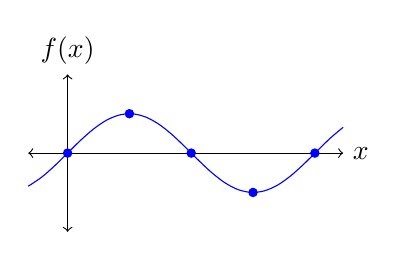
\begin{tikzpicture}[xscale=0.5,yscale=0.5]
        \draw[<->] (-1,0) -- (7,0) node[right] {$x$};
        \draw[<->] (0,-2) -- (0,2) node[above] {$f(x)$};
        \draw[scale=1,domain=-1:7,smooth,variable=\x,blue] plot ({\x},{sin(\x r)});
        \filldraw[blue] (0,0) circle[radius=3pt];
        \filldraw[blue] (3.14,0) circle[radius=3pt];
        \filldraw[blue] (1.57,1) circle[radius=3pt];
        \filldraw[blue] (6.28,0) circle[radius=3pt];
        \filldraw[blue] (4.71,-1) circle[radius=3pt];
    \end{tikzpicture} \hspace{\stretch{1}} $\to$ \hspace{\stretch{1}}
    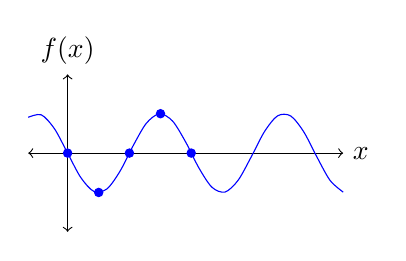
\begin{tikzpicture}[xscale=0.5,yscale=0.5]
        \draw[<->] (-1,0) -- (7,0) node[right] {$x$};
        \draw[<->] (0,-2) -- (0,2) node[above] {$f(x)$};
        \draw[scale=1,domain=-1:7,smooth,variable=\x,blue] plot ({\x},{-sin(2*\x r)});
        \filldraw[blue] (0,0) circle[radius=3pt];
        \filldraw[blue] (1.57,0) circle[radius=3pt];
        \filldraw[blue] (3.14,0) circle[radius=3pt];
        \filldraw[blue] (0.79,-1) circle[radius=3pt];
        \filldraw[blue] (2.36,1) circle[radius=3pt];
    \end{tikzpicture}
    \hspace{\stretch{1}}
\end{figure} $\Box$
\end{solution}
\begin{remark}
The graphs are shown at the top of the next page due to spacing limitations.
\end{remark}
Now that we have covered the two basic functions of sine and cosine, we can move on to the more complex trigonometric functions. We'll start with the tangent function, then move onto the three reciprocal functions.

If you remember back to \hyperlink{section.12.1}{Section 12.1}, the tangent functions is defined to be the ratio between the sine and the cosine of a given input angle: $\tan(x)=\dfrac{\sin(x)}{\cos(x)}$. Like all other special functions you've studied so far, there are a set of special points which need to be found when sketching the function. In the simplest case of just the parent function (without any transformations applied to it), you need to plot all of the zeros and all of the (vertical) asymptotes.

Since the tangent function is defined to be this ratio between the sine and cosine functions, zeros occur whenever the numerator $\sin⁡(x)=0$; likewise vertical asymptotes occur whenever the denominator $\cos⁡(x)=0$. Using the techniques developed in \hyperlink{section.12.3}{Section 12.3} we can solve these two equations. \begin{align*}
    \sin(x)=0 &\implies x=\pi k \hspace{12mm} k\in\mathbb{Z}\\ \cos(x)=0 &\implies x=\dfrac{\pi}{2}+\pi k \hspace{5mm} k\in\mathbb{Z}
\end{align*}
Thus, we now know the tangent function has zeros at every integer multiple of $\pi$, and that there are vertical asymptotes at every integer multiple of $\pi$, but offset by $\dfrac{\pi}{2}$.
\begin{wrapfigure}{r}{5cm}
    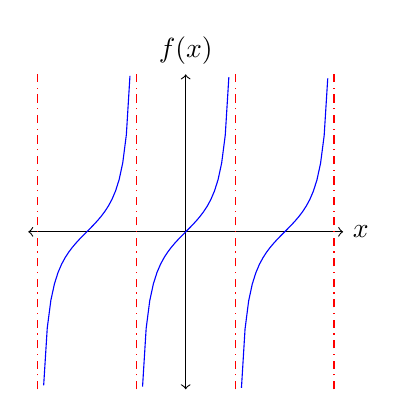
\begin{tikzpicture}[xscale=0.4,yscale=0.4]
        \draw[<->] (-5,0) -- (5,0) node[right] {$x$};
        \draw[<->] (0,-5) -- (0,5) node[above] {$f(x)$};
        \draw[scale=1,domain=-1.37:1.37,variable=\x,blue] plot ({\x},{tan(\x r)});
        \draw[scale=1,domain=1.77:4.51,variable=\x,blue] plot ({\x},{tan(\x r)});
        \draw[scale=1,domain=-4.51:-1.77,variable=\x,blue] plot ({\x},{tan(\x r)});
        \draw[dashdotted,red] (-1.57,-5) -- (-1.57,5);
        \draw[dashdotted,red] (1.57,-5) -- (1.57,5);
        \draw[dashdotted,red] (-4.71,-5) -- (-4.71,5);
        \draw[dashdotted,red] (4.71,-5) -- (4.71,5);
    \end{tikzpicture}
\end{wrapfigure}
To the right here is a graph of the tangent function in blue with zeros and vertical asymptotes of the function in red.

\begin{note}
Like the sine and cosine functions, you typically will only be asked to sketch one (maybe two) period(s) of the function. One period here is one of the chunks between any two adjacent asymptotes; for example, the interval $\left(-\dfrac{\pi}{2},\dfrac{\pi}{2}\right)$ represents one possible period of the function.
\end{note}

Introducing transformations to the tangent function is extremely similar to how it was done with the sine and cosine functions, and is arguably simpler. Again, here's the general formula for the tangent function with transformations: $$f(x)=A\tan\left(\dfrac{\pi}{T}\left(x-\pi\right)\right)+I; \hspace{10mm} \begin{matrix} A=\text{amplitude} & T=\text{period} \\ \phi=\text{phase shift} & I=\text{vertical shift} \end{matrix}.$$
While amplitude clearly affects how you sketch a sine or cosine wave, most teachers/professors wouldn't care if you drew $f(x)=\tan⁡(x)$ and $g(x)=2\tan⁡(x)$ the same. This stems from the fact that the "special features" of the tangent function (zeros and asymptotes) aren't affected numerically by scale factors. A negative scale factor, however, does change which way the graph curves (seen in Example 12.19).

Note the difference between the scale factor inside of the function for tangent and for sine ($\dfrac{\pi}{T}$ vs $\dfrac{2\pi}{T}$ respectively). This is because the period of the parent tangent function is half that of the parent sine/cosine function.

The variable change of the vertical shift from $E$ to $I$ is largely unimportant. The reasoning behind this is that the better expression for an "equilibrium point" within the context of the tangent function is an "inflection point," jargon from the field of Calculus. 
\begin{wrapfigure}{r}{5cm}
    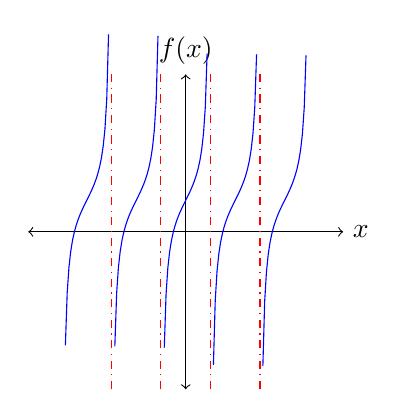
\begin{tikzpicture}[xscale=0.4,yscale=0.4]
        \draw[<->] (-5,0) -- (5,0) node[right] {$x$};
        \draw[<->] (0,-5) -- (0,5) node[above] {$f(x)$};
        \draw[scale=1,domain=-0.68:0.68,variable=\x,blue] plot ({\x},{tan(2*\x r)+1});
        \draw[scale=1,domain=0.88:2.25,variable=\x,blue] plot ({\x},{tan(2*\x r)+1});
        \draw[scale=1,domain=-2.25:-0.88,variable=\x,blue] plot ({\x},{tan(2*\x r)+1});
        \draw[scale=1,domain=3.82:2.45,variable=\x,blue] plot ({\x},{tan(2*\x r)+1});
        \draw[scale=1,domain=-2.45:-3.82,variable=\x,blue] plot ({\x},{tan(2*\x r)+1});
        \draw[dashdotted,red] (-0.79,-5) -- (-0.79,5);
        \draw[dashdotted,red] (0.79,-5) -- (0.79,5);
        \draw[dashdotted,red] (-2.36,-5) -- (-2.36,5);
        \draw[dashdotted,red] (2.36,-5) -- (2.36,5);
    \end{tikzpicture}
\end{wrapfigure}
\begin{example}
Sketch the function $f(x)=\tan(2x)+1$.
\end{example}
\begin{solution}
Since the input is being scaled by two, everything in the graph will be horizontally stretched by $\dfrac{1}{2}$. This means "inflection points" will occur at every integer multiple of $\dfrac{\pi}{2}$ and asymptotes at every integer multiple of $\dfrac{\pi}{2}$ with an offset of $\dfrac{\pi}{4}$.  The $+1$ simply shifts everything up one unit. $\Box$
\end{solution}
\begin{example}
Sketch the function $f(x)=-2\tan\left(2x+\dfrac{\pi}{4}\right)$.
\end{example}
\begin{wrapfigure}{r}{5cm}
    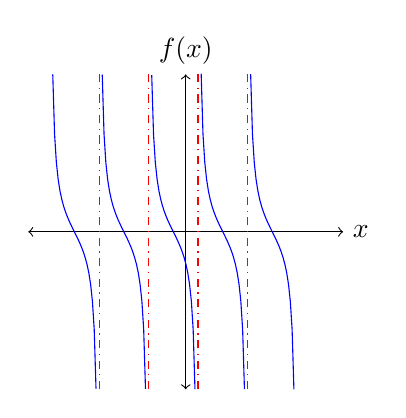
\begin{tikzpicture}[xscale=0.4,yscale=0.4]
        \draw[<->] (-5,0) -- (5,0) node[right] {$x$};
        \draw[<->] (0,-5) -- (0,5) node[above] {$f(x)$};
        \draw[scale=1,domain=-1.079:0.294,variable=\x,blue] plot ({\x},{-(tan(2*\x r)+1)/(1-tan(2*\x r)});
        \draw[scale=1,domain=0.491:1.865,variable=\x,blue] plot ({\x},{-(tan(2*\x r)+1)/(1-tan(2*\x r)});
        \draw[scale=1,domain=-2.65:-1.277,variable=\x,blue] plot ({\x},{-(tan(2*\x r)+1)/(1-tan(2*\x r)});
        \draw[scale=1,domain=2.062:3.436,variable=\x,blue] plot ({\x},{-(tan(2*\x r)+1)/(1-tan(2*\x r)});
        \draw[scale=1,domain=-4.221:-2.848,variable=\x,blue] plot ({\x},{-(tan(2*\x r)+1)/(1-tan(2*\x r)});
        \draw[dashdotted,red] (0.39,-5) -- (0.39,5);
        \draw[dashdotted,red] (-1.17,-5) -- (-1.17,5);
        \draw[dashdotted,red] (-2.747,-5) -- (-2.747,5);
        \draw[dashdotted,red] (1.96,-5) -- (1.96,5);
    \end{tikzpicture}
\end{wrapfigure}
\begin{solution}
Again, like in Example 12.17, we need to factor the input: $\tan\left(2x+\dfrac{\pi}{4}\right)=\tan\left(2\left(x+\dfrac{\pi}{8}\right)\right)$. Now we can break the function down into its transformations. Since we multiply the input the input by two, we first horizontally stretch the parent tangent function by $\dfrac{1}{2}$. Then we can follow up by applying the horizontal shift given by $\phi=-\dfrac{\pi}{8}$. Finally, we reflect everything over the $y$-axis due to the negative coefficient out front. \begin{align*}
    \text{Inflection Points}&: x=-\dfrac{\pi}{8}+\dfrac{\pi}{2}k;\hspace{3mm}k\in\mathbb{Z}\\
    \text{Asymptotes}&: x=\dfrac{\pi}{8}+\dfrac{\pi}{2}k;\hspace{3mm} k\in\mathbb{Z}
\end{align*} $\Box$
\end{solution}
Finally, we can finish with the three reciprocal functions $csc⁡(x)$, $sec⁡(x)$, and $cot⁡(x)$. The cosecant and secant functions are usually grouped together since they are visually very similar, just like the sine and cosine functions. There are three general rules for these reciprocal functions: \begin{itemize}
    \item 	Whenever you see a root (zero) in one of the normal trigonometric functions, there will be a vertical asymptote at the same locations in its corresponding reciprocal function.
	\item Whenever you see an extrema in one of the normal functions, you will see an extrema in the reciprocal function of the opposite type (min $\to$ max, max $to$ min).
	\item Whenever you see a vertical asymptote in one of the normal functions you will see a root (zero) in its corresponding reciprocal function.
\end{itemize}
\begin{figure}[!ht]
    \centering
    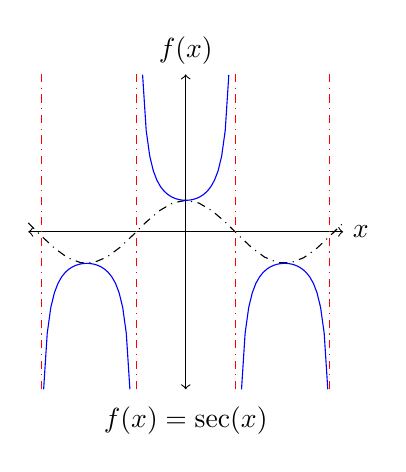
\begin{tikzpicture}[xscale=0.4,yscale=0.4]
        \draw[<->] (-5,0) -- (5,0) node[right] {$x$};
        \draw[<->] (0,-5) -- (0,5) node[above] {$f(x)$};
        \draw[scale=1,domain=-5:5,variable=\x,dashdotted] plot ({\x},{cos(\x r)});
        \draw[scale=1,domain=-1.369:1.369,variable=\x,blue] plot ({\x},{sec(\x r)});
        \draw[scale=1,domain=1.772:4.511,variable=\x,blue] plot ({\x},{sec(\x r)});
        \draw[scale=1,domain=-4.511:-1.772,variable=\x,blue] plot ({\x},{sec(\x r)});
        \draw[dashdotted,red] (1.57,-5) -- (1.57,5);
        \draw[dashdotted,red] (-1.57,-5) -- (-1.57,5);
        \draw[dashdotted,red] (-4.57,-5) -- (-4.57,5);
        \draw[dashdotted,red] (4.57,-5) -- (4.57,5);
        \draw (0,-6) node {$f(x)=\sec(x)$};
    \end{tikzpicture}
    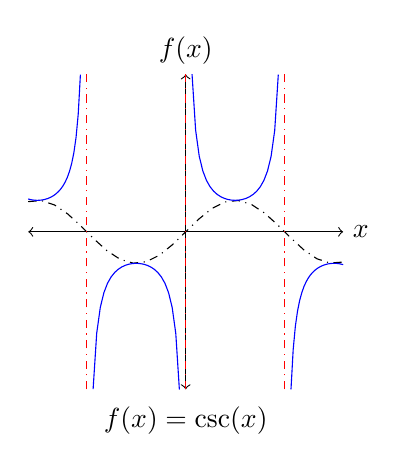
\begin{tikzpicture}[xscale=0.4,yscale=0.4]
        \draw[<->] (-5,0) -- (5,0) node[right] {$x$};
        \draw[<->] (0,-5) -- (0,5) node[above] {$f(x)$};
        \draw[scale=1,domain=-5:5,variable=\x,dashdotted] plot ({\x},{sin(\x r)});
        \draw[scale=1,domain=0.201:2.94,variable=\x,blue] plot ({\x},{1/(sin(\x r))});
        \draw[scale=1,domain=3.343:5,variable=\x,blue] plot ({\x},{1/(sin(\x r))});
        \draw[scale=1,domain=-5:-3.343,variable=\x,blue] plot ({\x},{1/(sin(\x r))});
        \draw[scale=1,domain=-2.94:-0.201,variable=\x,blue] plot ({\x},{1/(sin(\x r))});
        \draw[dashdotted,red] (3.14,-5) -- (3.14,5);
        \draw[dashdotted,red] (-3.14,-5) -- (-3.14,5);
        \draw[dashdotted,red] (0,-5) -- (0,5);
        \draw (0,-6) node {$f(x)=\csc(x)$};
    \end{tikzpicture}
    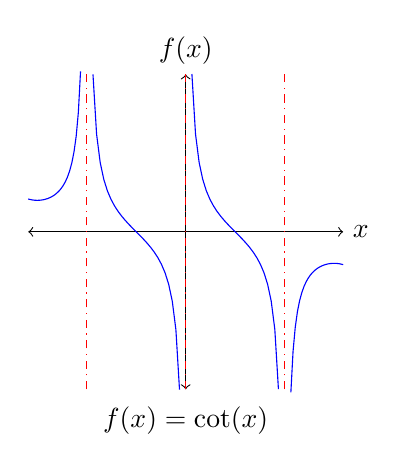
\begin{tikzpicture}[xscale=0.4,yscale=0.4]
        \draw[<->] (-5,0) -- (5,0) node[right] {$x$};
        \draw[<->] (0,-5) -- (0,5) node[above] {$f(x)$};
        \draw[scale=1,domain=0.197:2.944,variable=\x,blue] plot ({\x},{1/(tan(\x r))});
        \draw[scale=1,domain=-2.944:-0.197,variable=\x,blue] plot ({\x},{1/(tan(\x r))});
        \draw[scale=1,domain=-5:-3.339,variable=\x,blue] plot ({\x},{1/(sin(\x r))});
        \draw[scale=1,domain=3.339:5,variable=\x,blue] plot ({\x},{1/(sin(\x r))});
        \draw[dashdotted,red] (3.14,-5) -- (3.14,5);
        \draw[dashdotted,red] (-3.14,-5) -- (-3.14,5);
        \draw[dashdotted,red] (0,-5) -- (0,5);
        \draw (0,-6) node {$f(x)=\cot(x)$};
    \end{tikzpicture}
\end{figure}
Above are the three parent reciprocal functions $\csc⁡(x)$, $sec⁡(x)$, and $cot⁡(x)$.  In blue are the functions themselves, in red are all of the vertical asymptotes (and the inflection points for $cot⁡(x)$), and in black are the normal trigonometric functions for reference.
\begin{note}
It is often recommended (for sketching one of the reciprocal trigonometric functions) that you lightly draw the normal function as a reference (i.e. $\sin(x)$ should be drawn with $\csc(x)$.)
\end{note}

\begin{wrapfigure}{r}{5cm}
    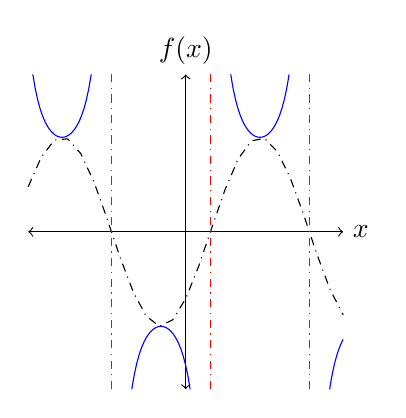
\begin{tikzpicture}[xscale=0.4,yscale=0.4]
        \draw[<->] (-5,0) -- (5,0) node[right] {$x$};
        \draw[<->] (0,-5) -- (0,5) node[above] {$f(x)$};
        \draw[scale=1,domain=-5:5,variable=\x,dashdotted] plot ({\x},{2.121*(sin(\x r)-cos(\x r))});
        \draw[scale=1,domain=-1.713:0.142,variable=\x,blue] plot ({\x},{6/(1.414*(sin(\x r)-cos(\x r)))});
        \draw[scale=1,domain=1.429:3.283,variable=\x,blue] plot ({\x},{6/(1.414*(sin(\x r)-cos(\x r)))});
        \draw[scale=1,domain=-4.854:-3,variable=\x,blue] plot ({\x},{6/(1.414*(sin(\x r)-cos(\x r)))});
        \draw[scale=1,domain=4.57:5,variable=\x,blue] plot ({\x},{6/(1.414*(sin(\x r)-cos(\x r)))});
        \draw[dashdotted,red] (3.92,-5) -- (3.92,5);
        \draw[dashdotted,red] (-2.36,-5) -- (-2.36,5);
        \draw[dashdotted,red] (0.79,-5) -- (0.79,5);
    \end{tikzpicture}
\end{wrapfigure}

In terms of transformations, they work the same as the original three trigonometric functions.

\begin{example}
Sketch the function $f(x)=3\csc\left(x-\dfrac{\pi}{4}\right)$.
\end{example}
\begin{solution}
We use the same color scheme as in the parent functions above.

We have two transformations here $-$ first a horizontal shift given by $\phi=\dfrac{\pi}{4}$, then a scale factor of $3$ vertically stretching the graph.
\begin{align*}
    \text{Asymptotes}&: x=\dfrac{\pi}{4}+\pi k;\hspace{3mm} k\in\mathbb{Z} \\
    \text{Extrema}&: x=\dfrac{\pi}{2}+\dfrac{\pi}{4}+\pi k=\dfrac{3\pi}{4}+\pi k;\hspace{3mm} k\in\mathbb{Z}
\end{align*} $\Box$
\end{solution}
We didn't include an example for each of the other since we believed it to be too repetitive.  So, this is where the section ends.  If you don't choose to read the last section (although we strongly encourage you do), you can move on to the Review and Challenge problems.
\section{Author's Note on Sinusoidal Curves}
\noindent In this section, we wanted to add on a note here to you the reader. We also wish to quickly stress that \textit{this section is not strictly necessary for any basic understanding of trigonometry}; you may proceed to the next chapter if you wish.

In writing this chapter, we were forced to think about my knowledge and experience with trigonometry throughout high school, and how we could present an introduction which someone with no prior familiarity to the subject could follow. One thing we realized was just how incomplete our understanding of sinusoidal curves/functions truly was. In every single math and physics class we took through high school we used $\sin⁡(x)$ in some capacity, yet seldom remember ever being told exactly what it is, what it does, and what defines it. That is the purpose of this section. Five definitions of the sine function and sinusoidal curves will be given here, each of which has its own advantages, disadvantages, and specific context for when they are typically used.

\begin{remark}
While the first two definitions have already been discussed in the previous two sections, the final three do involve complex mathematical ideas. While trigonometry and its ideas are deeply rooted in Calculus, the final definitions will be presented in a way in which no knowledge of Calculus is required.
\end{remark}

\textbf{Root Definition}. Let there be a right triangle with hypotenuse $1$ and some (non-right) angle within be denoted by $\theta$. $\sin(\theta)$ here is defined to be the length of the side of the triangle opposite $\theta$; whereas $\cos(\theta)$ is the length of the adjacent side.

\begin{wrapfigure}{r}{6cm}
    \begin{tikzpicture}[xscale=0.4,yscale=0.4]
        \draw (0,0) -- (10,0) -- (0,10) -- (0,0);
        \draw (-2,5) node {$\sin(\theta)$};
        \draw (5,-1) node {$\cos(\theta)$};
        \draw (8,1) node {$\theta$};
    \end{tikzpicture}
\end{wrapfigure}

This is the most basic definition for the sine and cosine functions. While it may be limited in utility due to a restricted domain, it helps as a starting point to learning more useful definitions.

\textbf{Base Definition}. Let there be a unit circle centered at the origin.  Given any angle $\theta$, a distinct point $P$ can be found by rotating around the circle $\theta$ radians.  If $\theta$ is positive, rotate

\begin{wrapfigure}{r}{6cm}
    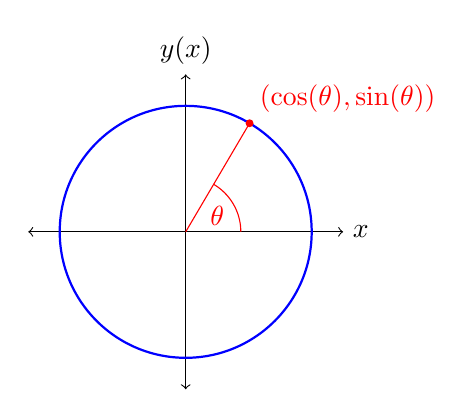
\begin{tikzpicture}[xscale=0.20,yscale=0.20]
      \draw[<->] (-10,0) -- (10,0) node[right] {$x$};
      \draw[<->] (0,-10) -- (0,10) node[above] {$y(x)$};
      \draw[blue,thick] (0,0) circle[radius=8];
      \draw[red] (0,0) -- (4.056,6.895);
      \filldraw[red,thick] (4.056,6.895) circle[radius=5pt] node[anchor=south west] {$(\cos(\theta),\sin(\theta))$};
      \draw[red] (2,1) node {$\theta$};
      \draw [red,domain=0:59.5] plot ({3.5*cos(\x)}, {3.5*sin(\x)});
    \end{tikzpicture}
\end{wrapfigure}

\noindent counterclockwise, if negative, clockwise.  (Start rotating from the point $(1,0)$). The Cartesian coordinates of $P$ are defined to be $(\cos(\theta),\sin(\theta))$.

This is the most commonly “referenced” definition of the two functions (at least in high school) as it provides the ability to fluidly transition between algebraic and geometric perspectives. A major advantage is that the domain is extended to $\mathbb{R}$.

\textbf{Function Analysis Definition}. Sinusoidal curves $-$ a family of curves $-$ can be defined as the only curves which follow the following two rules. $$f^2(x)+f^2(x+\phi)=c \hspace{5mm} (\phi,c\in\mathbb{R}).$$
Let's discuss what these two rules actually mean. The first is a generalization to an extremely important equation in trigonometry called The Pythagorean Identity. Using the diagram from the “root definition” and the Pythagorean theorem ($a^2+b^2=c^2$) it is easy to show: $$\sin^2(x)+\cos^2(x)=1.$$
Another important feature of the sine and cosine functions to notice is that each is simply a “shifted” version of the other. Put more precisely: $$\sin\left(x-\dfrac{\pi}{2}\right)=\cos(x).$$
While this idea is much more easily understood with the visual aid of a graph, a quick "proof" of this once again comes from the base definition. Using the fact that the sum of angles in a triangle equals π we can say the following about a right triangle: $\theta+\phi+\dfrac{\pi}{2}=\pi \implies \theta=\dfrac{\pi}{2}-\phi$. Since the opposite side to $\theta$ is the same side as the adjacent side to $\phi$ we can prove the above equation. Allowing for any frequency curve gives us the variable $\phi$ and any amplitude $-$ the variable $c$.

As for the second rule, let's start with the term continuous. Any function is non-continuous if there is a “break” in the curve, such as in the case of a piece-wise function. Therefore, it could be said that a function is “continuous everywhere” if the graph of the function could be drawn without ever having to pick up your pencil/pen. The term “differentiable” is essentially a jargon term from Calculus which in essence means “smooth.” For example $f(x)=|x|$ is not differentiable at $x=0$ since at that point there is a "sharp turn" where the graph is not smooth.

So, after boiling down these statements, we could translate everything into layman's terms: sinusoidal curves are the only curve which (1) could be drawn with a pencil without ever lifting the pencil up, (2) are smooth everywhere, and (3) follow a general form of The Pythagorean Identity.

\begin{remark}
As the authors of this book, we were unable to rigorously prove this definition to be consistent with all other definitions. We all have agreed, however, that this definition appears to be reasonable; we were additionally unable to come up with any counterexamples. We just want to make a disclaimer saying that while we cannot prove it, we conjecture the above to be true.
\end{remark}

\textbf{Physics / Differential Equations Definition}. While technically this definition is deeply rooted in Calculus, real-life applications in physics allows for us to skip all the details and get straight to the concepts. \textit{Simple Harmonic Motion} is a description in Physics for any object moving in a sinusoidal fashion. As an example, the most common case in which this comes up is with (ideal) horizontal springs.

\begin{wrapfigure}{r}{5cm}
    \begin{tikzpicture}
        \node[circle,fill=blue,inner sep=2.5mm] (a) at (0,0) {};
        \node[circle,fill=blue,inner sep=2.5mm] (b) at (2,2) {};
        \draw[decoration={aspect=0.3, segment length=3mm, amplitude=3mm,coil},decorate] (0,5) -- (a); 
        \draw[decoration={aspect=0.3, segment length=1.5mm, amplitude=3mm,coil},decorate] (2,5) -- (b); 
        \fill [pattern = north east lines] (-1,5) rectangle (3,5.2);
        \draw[thick] (-1,5) -- (3,5);
    \end{tikzpicture}
\end{wrapfigure}

Looking at the diagram to the right, if we pull the ball downward (left image) we know the ball will be pulled by the spring back to up; likewise, if the spring is pushed up (right image), the ball will want to be pushed back down. The more the spring is compressed or compressed, the more the spring will pull or push back $-$ equal and opposite in nature. In a single statement, we can say that the force the spring applies to the ball is always equal, but in opposite direction, to the ball's position: $a(t)=-x(t)$.

The standard sine curve is the solution to this equation which starts at $x=0$ and with an initial speed of $1$ unit per second in the positive $x$-direction; the cosine curve is the solution which starts at $x=1$ and with an initial speed of zero.

\begin{remark}
Here the independent variable here is $t$ for time, with the dependent variable being the position of the object.
\end{remark}

\textbf{Taylor Series Definition}.  This is arguably the most mathematically complex definition for the sine and cosine functions, they have to do with infinite sums. If you haven't been introduced to the concept yet, we'll start with something simple here. It's an understandably strange idea in math that you could add up infinitely many things but end up with a finite result. Let's take a look at a simple case. $$\sum_{n=0}^{\infty}{\left(\dfrac{1}{2}\right)^n}=1+\dfrac{1}{2}+\dfrac{1}{4}+\dfrac{1}{8}+\dfrac{1}{16}+\cdots=2.$$
At each step in the sum you half your current distance from $2$. While at any finite step you're always just short of $2$, mathematicians consider that at after summing these terms "infinitely" the total “equals” $2$. The idea behind a "Taylor Series" is to create a very specific infinite sum which equals a function. The derivation of these sums is a major topic within Calculus 2—something far beyond the goals of this book. The series for sine and cosine will be left here for those interested.
\begin{align*}
    \sum_{n=0}^{\infty}{\dfrac{(-1)^n}{(2n+1)!}x^{2n+1}}&=x-\dfrac{x^3}{3!}+\dfrac{x^5}{5!}-\dfrac{x^7}{7!}+\dfrac{x^9}{9!}-\cdots=\sin(x) \\
    \sum_{n=0}^{\infty}{\dfrac{(-1)^n}{(2n)!}x^{2n}}&=1-\dfrac{x^2}{2!}+\dfrac{x^4}{4!}-\dfrac{x^6}{6!}+\dfrac{x^8}{8!}-\cdots=\cos(x)    
\end{align*}
With this, we end the chapter.  This chapter has been quite lengthy and has covered a lot of material, but understanding this chapter will greatly help your time in Pre-calculus.  A quarter of the curriculum is trigonometry; with this preview, you should be well on your way to success.

Give the problems a try! The challenge problems get somewhat difficult, but we believe you can do it!
\begin{reviewset}
\item Evaluate each of the following: (as an extra challenge, try finding them in your head, without writing anything down.) \newline
(a) $\cos(150^{\circ})$ \hspace{\stretch{1}} (c) $\csc(90^{\circ})$ \hspace{\stretch{1}} (e) $\cos(315^{\circ})$ \hspace{\stretch{1}} (g) $\sin(-120^{\circ})$ \newline
(b) $\tan(270^{\circ})$ \hspace{\stretch{1}} (d) $\sin(225^{\circ})$ \hspace{\stretch{1}} (f) $\tan(30^{\circ})$ \hspace{\stretch{1}} (h) $\cos(-540^{\circ})$ \vspace{3mm}
\item Evaluate each of the following: (as an extra challenge, try finding them in your head, without writing anything down.) \newline
(a) $\cos\left(\dfrac{3\pi}{4}\right)$ \hspace{\stretch{1}} (b) $\sin\left(-\pi\right)$ \hspace{\stretch{1}} (c) $\cot\left(\dfrac{5\pi}{4}\right)$ \hspace{\stretch{1}} (d) $\sec\left(\dfrac{7\pi}{6}\right)$ \vspace{3mm}
\item What are the domain and range of the function $f(t)=2\tan(3t-\pi)$? \vspace{3mm}
\item For how many values of $x$ such that $0\leq x\leq 7\pi$ is $\cos(x)=-0.01$? \vspace{3mm}
\item Find the amplitude, period, and phase shift of $f(x)=-2\sin\left(\dfrac{x}{4}-\dfrac{\pi}{3}\right)$. \vspace{3mm}
\item Find all values of $k$ such that $3\cot(4k-\pi)=\sqrt{3}$. \vspace{3mm}
\item How is the graph of $\sin\left(x-\dfrac{\pi}{2}\right)$ related to the graph of $y(x)=\cos(x)$? What about $\sin\left(x+\dfrac{\pi}{2}\right)$? \vspace{3mm}
\item Cole is writing a calculator program that contains the following lines of code: \begin{center}\texttt{x = t*sin(y)}.\end{center}  The line of code sets $x$ equal to the product of $t$ and the sine of $y$.  Unfortunately, $y$ is in degrees, and the "sin" function in her program expects it to be radians.  How can Cole change this line of code to obtain the desired result? \vspace{3mm}
\item Graph $y(x)=2\sin\left(\dfrac{2x}{3}-\pi\right)$. \vspace{3mm}
\item Joshua was taking a Pre-calculus test and was asked to find $\tan(40^{\circ})$. He used his calculator to find the answer by typing in $40$ and pressing the tangent key. He wrote down what his calculator told him, $-1.11721$. He was rather upset to have his answer marked incorrect and was convinced his calculator was broken. \newline 
(a) Even without knowing what $\tan(40^{\circ})$ equals, how should Joshua have known that his answer of $-1.11721$ was not the correct answer? \newline 
(b) What mistake did he probably make? \vspace{3mm}
\end{reviewset}
\begin{challengeset}
\item If $8\tan(\theta)=3\cos(\theta)$, where $0<\theta<\pi$, determine the value of $\sin(\theta)$. \vspace{3mm}
\item The graph of some function $h(x)=\sin(px+q)$ is shown below for some values of $p$ and $q$. The resulting graph is shown below.

\begin{figure}[!ht]
    \centering
    \begin{tikzpicture}[xscale=0.7,yscale=0.7]
        \draw[<->] (-10,0) -- (10,0) node[right] {$x$};
        \draw[<->] (0,-2) -- (0,2) node[above] {$f(x)$};
        \draw [blue,domain=-10:10,variable=\x,smooth] plot ({\x}, {(sin(4*\x/3 r)*1.73-cos(4*\x/3 r))/2});
        \foreach \x in {-7.85,-6.28,-4.71,-3.14,-1.57,1.57,3.14,4.71,6.28,7.85}
        \draw[shift={(\x,0)},color=black] (0pt,3pt) -- (0pt,-3pt);
        \draw (-7.85,0) node[below=0.5mm] {$-\frac{5\pi}{2}$};
        \draw (-6.28,0) node[below=0.5mm] {$-2\pi$};
        \draw (-4.71,0) node[below=0.5mm] {$-\frac{3\pi}{2}$};
        \draw (-3.14,0) node[below=0.5mm] {$-\pi$};
        \draw (-1.57,0) node[below=0.5mm] {$-\frac{\pi}{2}$};
        \draw (7.85,0) node[below=0.5mm] {$\frac{5\pi}{2}$};
        \draw (6.28,0) node[below=0.5mm] {$2\pi$};
        \draw (4.71,0) node[below=0.5mm] {$\frac{3\pi}{2}$};
        \draw (3.14,0) node[below=0.5mm] {$\pi$};
        \draw (1.57,0) node[below=0.5mm] {$\frac{\pi}{2}$};
        \draw[color=black] (3pt,1) -- (-3pt,1);
        \draw[color=black] (3pt,-1) -- (-3pt,-1);
    \end{tikzpicture}
\end{figure}

Determine all possible values of $p$ and $q$. (NOTE: the graph should be smoother, but there was trouble with graphing this one.) \vspace{3mm}
\item Find all values of $\theta$ such that $\sin(3\theta)<\dfrac{1}{2}$. (You don't need Chapter 15 for this one!) \vspace{3mm}
\item Consider a function $\arcsin(x)$ that is to be defined as the inverse of $\sin(x)$ over their respective domain and ranges.  Using your knowledge of trigonometric functions and inverse functions, answer the following questions: \newline 
(a) Evaluate $\arcsin(-1)$. \hspace{\stretch{1}} (c) Graph $\arcsin(x)$. \hspace{\stretch{1}} \newline 
(b) Give the domain and range of $\arcsin(x)$. \hspace{\stretch{1}} (d) Compute $\tan(\arcsin(0.5))$. \hspace{\stretch{1}}\vspace{3mm}
\item Is the function $f(x)=2\sin(x)-\tan(x)$ periodic? If so, what is the period? \vspace{3mm}
\end{challengeset}
\end{document}